\documentclass[11pt,twoside,a4paper]{article}

\usepackage[utf8]{inputenc}
\usepackage[T1]{fontenc}
\usepackage[brazil]{babel}
\usepackage[pdftex]{graphicx} 
\usepackage{amsmath}
\usepackage{amssymb}
\usepackage{amsthm}
\usepackage{mathabx}
\usepackage{indentfirst}
\usepackage{setspace}
\usepackage[usenames,svgnames,dvipsnames]{xcolor}
\usepackage[fixlanguage]{babelbib}
\usepackage[round,sort,nonamebreak]{natbib} % citação bibliográfica textual(plainnat-ime.bst)

\usepackage[pdftex,plainpages=false,pdfpagelabels,pagebackref,colorlinks=true,citecolor=DarkGreen,linkcolor=NavyBlue,urlcolor=DarkRed,filecolor=green,bookmarksopen=true]{hyperref}
\usepackage[all]{hypcap} 


\frenchspacing
\urlstyle{same}
\makeindex
\raggedbottom
%\fontsize{60}{62}\usefont{OT1}{cmr}{m}{n}{\selectfont}
%\cleardoublepage
\normalsize

\newcommand{\CC}{\mathcal{C}}
\newcommand{\LL}{\mathcal{L}}
\newcommand{\MM}{\mathcal{M}}
\newcommand{\PP}{\mathcal{P}}
\newcommand{\TT}{\mathcal{T}}

\newcommand{\N}{{\mathbb{N}}}
\newcommand{\Nb}{{\widebar{\N}}}
\newcommand{\Nz}{{\mathbb{N^*}}}
\newcommand{\Nzb}{{\mathbb{\widebar{N}^*}}}
\newcommand{\Z}{{\mathbb{Z}}}
\newcommand{\R}{{\mathbb{R}}}
\newcommand{\E}{{\mathbb{E}}}
\newcommand{\ind}{{\mathbb{I}}}
\newcommand{\diam}{{\mathrm{diam}}}
\newcommand{\var}{\mathop{\mathrm{Var}}}

\newtheorem{teorema}{Teorema}[section]
\newtheorem{lema}[teorema]{Lema}
\newtheorem{proposicao}[teorema]{Proposição}
\newtheorem{corolario}[teorema]{Corolário}


\author{Gabriel Ribeiro da Cruz Peixoto}
\title{Processo K não homogêneo - Construção e Taxas de transição}
\date{\today}

\begin{document}

\maketitle

\section{Definições}
\label{sec:definicoes}

Tomemos $\Nz = \{ 1, 2, 3, \ldots\}$. A esse conjunto adicionaremos um
novo símbolo, que denotaremos por $\infty$. Chamaremos esse novo
conjunto de $\Nzb$.

O processo K será um processo estocástico em tempo contínuo, cujo
espaço de estados será $\Nzb$. Chamaremos os elementos de $\Nzb$ de
estados ou sítios do processo.

Como parâmetros do processo, teremos uma família de números reais
estritamente positivos, $\{ \gamma_x, \lambda_x$, $x \in \Nz\}$. Além de
uma constante $c \in [0, \infty)$.  Para um estado $x \in \Nz$,
podemos interpretar $\gamma_x$ como o tempo médio para o processo sair
de $x$ e $\lambda_x$ vai controlar a taxa com que o processo tende a
entrar em $x$. Enquanto que $c$ controla o tempo em que o estado fica
em $\infty$.

Seguindo \cite{fontes:08}, iremos definir o processo K através de uma
construção. Adaptaremos levemente a construção descrita lá, para
permitir que estados tenham diferentes ``pesos'' (os $\lambda_x$).  O
espaço de probabilidade, $\Omega$, onde iremos construir o processo
será um espaço que admita as seguintes famílias de variáveis
aleatórias independentes:

\begin{itemize}
\item $\{ N_x: x \in \Nz \}$: processos pontuais de Poisson
  independentes, onde $N_x$ tem taxa $\lambda_x$ para cada $x \in \N$.
\item $\{T_n^x: x \in \Nzb , \, n = 0, 1, 2, 3, \ldots \}$: variáveis
  aleatórias exponencias de média $1$.
\end{itemize}

Para $t \geq 0$, iremos denotar por $N_x(t)$ o número de marcas do
processo de poisson $N_x$ no intervalo $[0, t]$, marcas essas que
iremos denotar por $0 \leq \sigma_1^x < \sigma_2^x < \ldots$ .

Agora podemos definir uma função aleatória que será nossa principal
ferramenta para trabalhar com esse processo. Para $t \geq 0$ e $y \in
\Nzb$, sob a convenção que $\gamma_\infty = 0$:

\begin{equation}
  \label{def:Gamma}
  \Gamma(t) = \Gamma^y_c (t) =
  ct +
  \gamma_y T_0^y +
  \sum_{x \in \N} \sum_{i = 1}^{N_x(t)}
  \gamma_x T_i^x
\end{equation}

Por convenção, considere que $\sum_{i=1}^{0}( \bullet ) = 0$.

Vamos impor uma restrição que garanta que $\Gamma$ seja quase
certamente finita para todo $t \in \R^+$:
\begin{equation}
  \sum_{x \in \Nz} \lambda_x\gamma_x < +\infty.
\end{equation}

Chamaremos o processo K iniciado em $y \in \Nb$ de $X^y_c$. Ele é
definido, para $t \geq 0$, da seguinte forma:

\begin{equation}
  \label{def:procK}
  X(t) = X^y_c (t) =
  \begin{cases}
    y, & \textrm{ se }  t < \gamma_y T_0^y\\
    x, & \textrm{ se } \Gamma^y_c(\sigma_i^x-) \leq t <
    \Gamma^y_c(\sigma^x_i)
    \textrm{ para algum } i \\
    \infty, & \textrm{ caso contrário.}
  \end{cases}
\end{equation}

Agora vamos enunciar dois resultados sobre o processo K que já haviam
sido provados em \cite{fontes:08}. Lá foi tratado apenas o caso
$\lambda_x = 1$ para todo $x \in \Nz$. Mas as demonstrações podem ser
transportadas diretamente para o caso não homogêneo.

\begin{teorema}
  O processo K quase certamente tem tragetórias Càdlàg. Isso é,
  contínuas à direita e com limites à esquerda.
\end{teorema}

\begin{teorema}
  O processo K é um processo fortemente Markoviano.
\end{teorema}



\section{Visualização}
\label{sec:visualizacao}

Para essa seção, vamos supor que $\sum_{x \in \Nz} \lambda_x <
\infty$. Nesse caso a sobreposição de todos os processos de Poisson
$\{N_x : x \in \Nz\}$ será um processo de Poisson de taxa $\sum_{x \in
  \Nz} \lambda_x < \infty$. Assim podemos quase certamente enumerar as
marcas desse processo de Poisson, denotando-as por $ \sigma_1 < \sigma_2 <
\ldots$.

O gráfico de $\Gamma$, fora das marcas $\sigma_1, \sigma_2,
\ldots$ é uma reta de inclinação $c$, e nas marcas
essa função tem dá saltos, de tamanho $\gamma_x T^x_i$, para algum $x$
e algum $i$. A Figura \ref{fig:graf_gamma} ilustra uma possível
realização de $\Gamma$.


Pela nossa construção, esses saltos corresponderão ao tempo que o
processso passa nos estados de $\Nz$, enquanto que no resto do tempo
ele está no $\infty$.

Assim nosso processo K se reduzirá a um processo Markoviano de
saltos. Vamos descreve-lo, separando nos casos $c = 0$ e $c > 0$.

Caso $c > 0$, $X^y_c(0) = y$ para todo $y \in \Nzb$, e estando em um
estado $x \in \Nz$, o processo esperará um tempo exponencial de média
$\gamma_x$para pular para o $\infty$.
Quano o processo estiver no $\infty$, ele esperará um tempo
exponencial de taxa $\sum_{x \in \Nz} \frac{\lambda_x}{c}$ para
pular. O destino desse salto será escolhido com probabilidade
proporcional às $\lambda_x$.

No caso $c=0$, teremos que $X^y_0(0) = y$ se $y \in \Nz$ e
$P(X^\infty_0(0) = z) = \frac{\lambda_z}{\sum_{x\in\Nz} \lambda_x}$
para todo $z \in \Nz$.  Estando em um estado $x$, o processo espera um
tempo exponencial de média $\gamma_x$ e depois pula para um estado $z
\in \Nzb$ com probabilidade $\frac{\lambda_z}{\sum_{x\in\Nz}
  \lambda_x}$.  Note que nesse caso nós nunca visitamos o $\infty$,
vale até mesmo que $X^\infty(0) \neq \infty$ quase certamente.


\begin{figure}
  \centering
  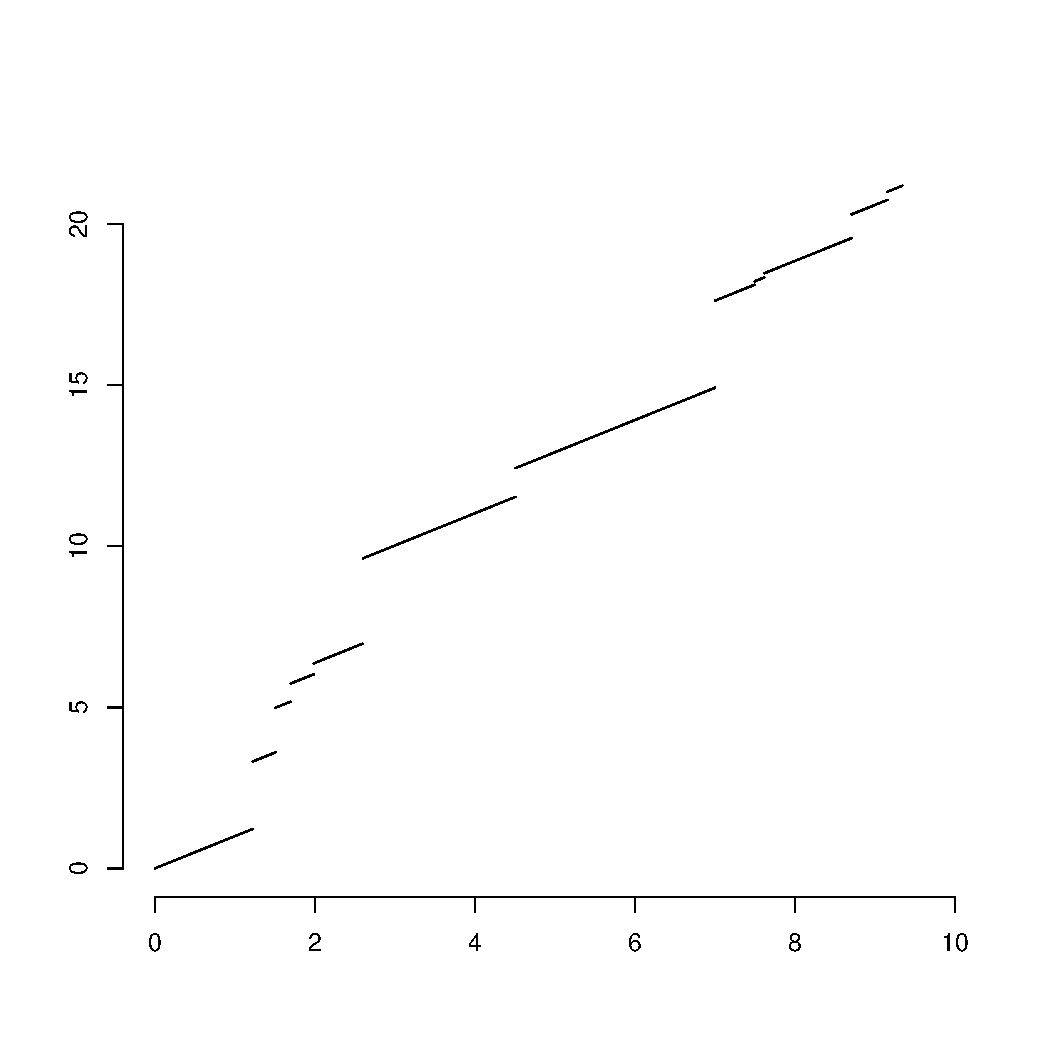
\includegraphics[width=.80\textwidth]{graf_gamma}
  \caption{Um exemplo de realização de $\Gamma$ quando $\sum_{x \in
      \Nz} \lambda_x < \infty$}
  \label{fig:graf_gamma}
\end{figure}

\section{Topologia sobre o espaço de estados}
\label{sec:topologia}

Será útil para alguns resultados munirmos $\Nzb$ de uma
topologia. Para isso considere a seguinte métrica:
\begin{equation}
  \label{eq:metrica}
  d(x, y) = \left\lvert \frac{1}{x} - \frac{1}{y} \right\rvert,
\end{equation}
para $x, y \in \Nzb$, sob a convenção de que $\frac{1}{\infty} = 0$.

Essa métrica induz uma topologia bastante natural, onde todos os
pontos $x \in \Nz$ são pontos isolados, e uma sequência converge ao
$\infty$ nessa topologia se ela divergir para infinito da maneira
usual.

Uma função $f: \Nzb \to \R$ será contínua se e somente se
$f(\infty) = \lim_{x \to \infty} f(x)$.

Vale ainda que essa topologia é compacta, nos dando boas propriedades
para trabalhar.

\section{Taxas de transição}

Para $x, y \in \Nzb$, $t \geq 0$, vamos definir:
\begin{equation}
  p_{xy} (t) = P(X^x(t) = y).
\end{equation}

E vamos denotar por $P(t)$ a ``matriz'' com entradas $p_{x y}(t)$. Boa
parte do trabalho nesse projeto de mestrado foi calcular a matriz de
derivadas de $P(t)$, definida por:

\begin{displaymath}
  Q = \lim_{t \searrow 0} \frac{P(t) - I}{t} 
\end{displaymath}.

Caso $c > 0$, essa matriz vale:
\begin{displaymath}
  Q = \left(
    \begin{array}{ccccc}
      -\frac{1}{\gamma_1} & 0 & 0 & \cdots & \frac{1}{\gamma_1}\\
      0 & -\frac{1}{\gamma_2} & 0 & \cdots & \frac{1}{\gamma_2}\\
      0 & 0 & -\frac{1}{\gamma_3} & \cdots & \frac{1}{\gamma_3}\\
      \vdots & \vdots & \vdots & \ddots & \vdots \\
      \frac{\lambda_1}{c} & \frac{\lambda_2}{c} &
      \frac{\lambda_3}{c} & \cdots & -\infty\\
    \end{array}
  \right).
\end{displaymath}

Equanto que no caso $c=0$, teremos:
\begin{displaymath}
  Q = \left(
    \begin{array}{ccccc}
      -\frac{1}{\gamma_1} & 0 & 0 & \cdots & 0\\
      0 & -\frac{1}{\gamma_2} & 0 & \cdots & 0\\
      0 & 0 & -\frac{1}{\gamma_3} & \cdots & 0\\
      \vdots & \vdots & \vdots & \ddots & \vdots \\
      \infty & \infty & \infty & \cdots & -\infty\\
    \end{array}
  \right).
\end{displaymath}

\section{Medida invariante}
\label{sec:invariante}

Tendo as taxas de transição calculadas, conseguimos mostrar que o
processo K tem uma única probabilidade invariante, dada por:
\begin{equation}
  \label{eq:invariante}
  \pi(x) = \begin{cases}
    \frac{\lambda_x \gamma_x}{c + \sum_{y \in \Nz} \lambda_y \gamma_y}
    & \textrm{ se } x \in \Nz \\
    \frac{c}{c + \sum_{y \in \Nz} \lambda_y \gamma_y}
    & \textrm{ se } x = \infty \\
  \end{cases}
\end{equation}


\section{Tempo passado no infinito}

\begin{teorema}
  Para todo $t > 0$, quase certamente, $c > 0$ se e somente se 
  \begin{displaymath}
    \int_0^t \ind (X^\infty_c(s) = \infty) ds > 0.
  \end{displaymath}
\end{teorema}

Como o tempo em que passamos no infinito, no caso $c = 0$, tem medida
de Lebesgue zero, faz sentido perguntar qual a dimensão de Hausdorf
desse conjunto.

\begin{teorema}
  $\Gamma(t)$, quando enxergada como um processo estocástico, é um
  subordinador. Isso é, é um processo estocastico não decrescente,
  contínuo à direita, que tem incrementos estacionários e independentes.
\end{teorema}

\begin{proposicao}
  O expoente de Laplace de $\Gamma^\infty_0(\bullet)$, vale:
  \begin{equation}
    \label{eq:exp-laplace}
    \Phi(u) = 
    u \sum_{x \in \Nz} \frac{\lambda_x \gamma_x}{1 + u \gamma_x}
  \end{equation}
\end{proposicao}

Como o tempo que o processo passa no $\infty$ é igual à imagem de
$\Gamma$, usando o Corolário 5.3 de \cite{bertoin:97}, obteremos que a
dimensão de Hausdorf desse cojunto é dada por:

\begin{equation}
  \label{eq:dim-hausdorf}
  \liminf_{u \to \infty} \frac{\log \Phi(u)}{\log u} 
\end{equation}

\begin{proposicao}
  Suponha que $\sup_{x\in\Nz}\lambda_x < \infty$ e que existam um
  $\delta>0$ e um $n_0 \in \Nz$ tal que $\gamma_x \leq x^{-(1+\delta)}$
  para todo $x > n_0$. Nessas condições:
  \begin{equation}
    \liminf_{u \to \infty} \frac{\log \Phi(u)}{\log u}  \leq \frac{1}{1+\delta}
  \end{equation}
\end{proposicao}

\begin{proposicao}
  Suponha que $\inf_{x\in\Nz}\lambda_x  > 0$ e que existam um
  $\delta>0$ e um $n_0 \in \Nz$ tal que $\gamma_x \geq x^{-(1+\delta)}$
  para todo $x > n_0$. Nessas condições:
  \begin{equation}
    \liminf_{u \to \infty} \frac{\log \Phi(u)}{\log u}  \geq \frac{1}{1+\delta}
  \end{equation}
\end{proposicao}

Assim, podemos fazer a dimensão de Hausdorf do processo K, no caso $c
= 0$ variar por qualquer valor no intervalo $[0, 1)$.


% ---------------------------------------------------------------------------- %
% Bibliografia
\singlespacing   % espaçamento simples
\bibliographystyle{plainnat-ime} % citação bibliográfica textual
\bibliography{../bibliografia}  % associado ao arquivo: 'bibliografia.bib'

\end{document}
